% ### Uses XeLaTeX ### %
% ### Needs beamer-master ### %
\documentclass[aspectratio=169]{beamer} %. Aspect Ratio 16:9
\usetheme{AI2} % beamerthemeSprace.sty
% DATA FOR FOOTER
\date{2019}
\title{}
\author{}
\institute{Advanced Institute for Artificial Intelligence (AI2)}
\begin{document}    
% ####################################
% FIRST SLIDE 						:: \SliTit{<Title of the Talk>}{<Author Name>}{<Intitution>}
% SLIDE SUB-TITLE					:: \SliSubTit{<Title of the Chapter>}{<Title of the Section>}
% SLIDE WITH TITLE 					:: \SliT{<Title>}{Content}
% SLIDE NO TITLE 						:: \Sli{<Content>} 
% SLIDE DOUBLE COLUMN WITH TITLE 	:: \SliDT{<Title>}{<First Column>}{<Second Column>}
% SLIDE DOUBLE COLUMN NO TITLE 		:: \SliD{<First Column>}{<Second Column>}
% SLIDE ADVANCED WITH TITLE 			:: \SliAdvT{<Title>}{<Content>}
% SLIDE ADVANCED  NO TITLE 			:: \SliAdv{<Content>}
% SLIDE ADVANCED DOUBLE TITLE 		:: SliAdvDT{<Title>}{<First Column>}{<Second Column>}
% SLIDE ADVANCED DOUBLE NO TITLE 	:: SliAdvD{<First Column>}{<Second Column>}
% ITEMIZE 							:: \begin{itemize}  \IteOne{1st Level} \IteTwo {2nd Level} \IteThr{3rd Level} \end{itemize}
% SECTION 							:: \secx{Section} | \secxx{Sub-Section}
% COLOR BOX 						:: \blu{blue} + \red{red} + \yel{yellow} + \gre{green}
% FRAME 							:: \fra{sprace} \frab{blue} \frar{red} + \fray{yellow} + \frag{green}	
% REFERENCE						:: \refer{<doi number>}
% FIGURE 							::  \img{X}{Y}{<scale>}{Figures/.png} 
% FIGURE							:: \begin{center}\includegraphics[scale=<#>]{Figures/.png}\end{center}
% PROJECT STATUS					:: \planned\~    \started\~   \underway\~   \done\~   
% EXERCICIO							:: \Exe{<#>}{<text>}
% STACKREL							:: \underset{<down>}{<up>}
% FLUSH LEFT						:: \begin{flalign*}  & <1st equation> & \\  & <12nd equation>  & \\ \end{flalign*}
% REAL / IMAGINAY					:: \Re / \Im
% SLASH								:: \sl{} or \sl
% BOLD MATH							:: \pmb{<>}
% ####################################
%
% FIRST SLIDE :: DO NOT BREAK LINE !!!
\SliTit{Numpy}{Advanced Institute for Artificial Intelligence}{https://advancedinstitute.ai}

% SLIDE WITH TITLE
\SliT{Sumario}{

\begin{itemize}
  \IteOne{Introdução}
  \IteOne{Estruturas}
  \IteOne{Atributos}
  \IteOne{Operações}
\end{itemize}

}

% SLIDE WITH TITLE
\SliT{Introdução}{

\begin{itemize}
  \IteOne{Biblioteca de computação científica}
  \IteOne{Especializada para trabalhar com matrizes}
  \IteOne{Funções de Álgebra Linear}
\end{itemize}

}

% SLIDE WITH TITLE
\SliT{Numpy}{

Numpy manipula classes do tipo:  ndarray
\begin{itemize}
  \IteOne{Representa a estrutura fornecida pelo Numpy}
  \IteOne{Estrutura parecida com as Listas}
  \IteOne{Classe possui diversos atributos e funções}
\end{itemize}

}

\SliT{Numpy}{

Alguns atributos:

\begin{itemize}
  \IteOne{ndarray.ndim - Numero de dimensões do array}
  \IteOne{ndarray.shape - Tupla com o tamanho dos array que representa cada
dimensão}
  \IteOne{ndarray.size - Quantidade de elementos no array}
  \IteOne{ndarray.dtype - Tipo de dados que estão armazenados no array}
\end{itemize}

}

\SliT{Numpy}{

Funções para criação de matrizes:

\begin{itemize}
  \IteOne{numpy.arange - Cria um array com valores sequenciais (similar a função range)}
  \IteOne{numpy.array - Convert outro objeto (list,tupla, etc) para ndarray}
  \IteOne{numpy.identity - cria matriz identidade de tamanho n}
  \IteOne{numpy.ones - cria matriz de tamanho n apenas com valores 1}
  \IteOne{numpy.zeros - cria matriz de tamanho n apenas com valores 0}
\end{itemize}

}

\SliT{Numpy}{

Algumas operações:

\begin{itemize}
  \IteOne{numpy.sum - Soma os valores de um array para uma determinada dimensão}
  \IteOne{numpy.prod - Multiplica os valores de um array para uma determinada dimensão}
  \IteOne{numpy.cumsum - Soma cumulativa dos valores de um array para uma determinada
dimensão}
  \IteOne{numpy.cumprod - Multiplicação cumulativa dos valores de um array para uma determinada
dimensão}

\end{itemize}

}

\SliT{Numpy}{

Algumas operações:

\begin{itemize}
  \IteOne{numpy.transpose - retorna a matriz transposta}
  \IteOne{numpy.dot - multiplica duas matrizes}
  \IteOne{numpy.reshape - alterar o formato da matriz, dentro de um mesmo conjunto de elementos}
  \IteTwo{ex: alterar o formato de 3x3 para 1x9, 4x4 para 2x8}

\end{itemize}

}

\SliT{Numpy}{

axis são definidos para matrizes com mais de uma dimensão. 

\begin{itemize}
  \IteOne{Uma matriz bidimensional possui dois eixos correspondentes:}
  \IteTwo{O primeiro correndo verticalmente para baixo nas linhas (eixo 0)}
  \IteTwo{O segundo correndo horizontalmente nas colunas (eixo 1)}
\end{itemize}

Exemplo:

\begin{itemize}
  \IteOne{somar cada linha de uma matriz}
  \IteTwo{usamos a operação sum com opcional axis=0}
  \IteOne{somar cada coluna de uma matriz}
  \IteTwo{usamos a operação sum com opcional axis=1}
\end{itemize}

}

\SliT{Numpy}{
\begin{center}
    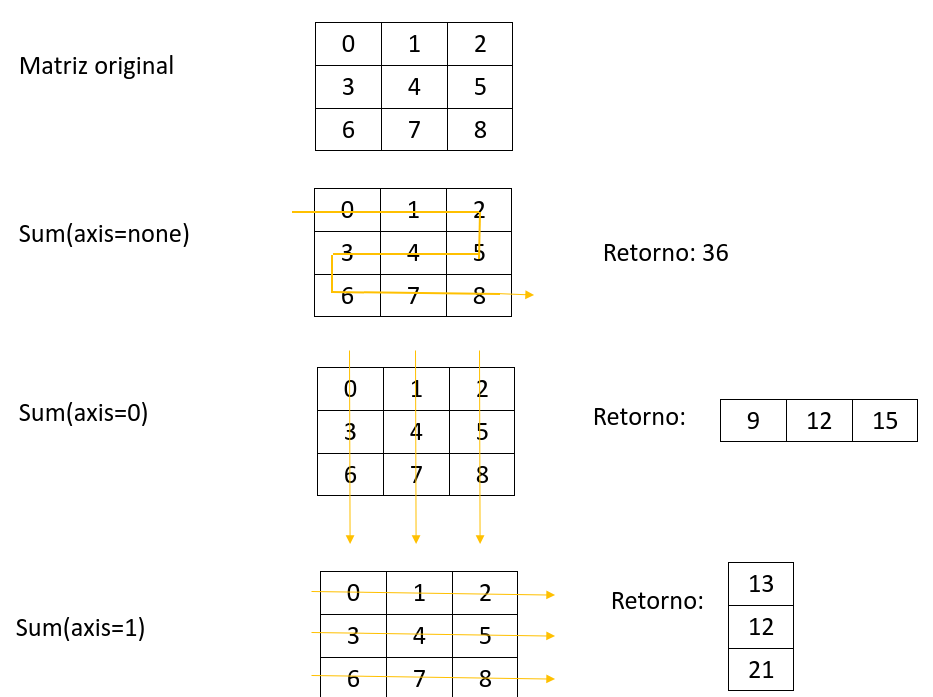
\includegraphics[scale=0.27]{axis.png}     
    \end{center}
}

\end{document}